\documentclass{whiteboard}
\begin{document}
\begin{frame}[plain,t]
\bbcover{Grafos}{Algoritmo de Prim}{Prof. Edson Alves}{Faculdade UnB Gama}

\end{frame}
\begin{frame}[plain,t]
\begin{tikzpicture}
\node[draw,opacity=0] at (0, 0) {x};
\node[draw,opacity=0] at (14, 8) {x};

	\node[anchor=west] (title) at (0.0, 7.0) { \Large \bbbold{Proponentes} };

	\node[] (jarnik) at (2.0, 4.0) { \includegraphics[scale=0.4]{figs/jarnik.jpg} };

	\node[] (jname) at (2.0, 1.0) { \bbbold{Vojtěch Jarník} };

	\node[] (jdate) at (2.0, 0.5) { \bbtext{(1930)} };

	\node[] (prim) at (7.0, 4.0) { \includegraphics[scale=1.3]{figs/prim.jpg} };

	\node[] (pname) at (7.0, 1.0) { \bbbold{Robert Clay Prim} };

	\node[] (pdate) at (7.0, 0.5) { \bbtext{(1957)} };

	\node[] (dijkstra) at (12.0, 4.0) { \includegraphics[scale=0.4]{figs/dijkstra.jpg} };

	\node[] (dname) at (12.0, 1.0) { \bbbold{Edsger Wybe Dijkstra} };

	\node[] (ddate) at (12.0, 0.5) { \bbtext{(1959)} };

\end{tikzpicture}
\end{frame}
\begin{frame}[plain,t]
\begin{tikzpicture}
\node[draw,opacity=0] at (0, 0) {x};
\node[draw,opacity=0] at (14, 8) {x};

	\node[anchor=west] (title) at (0.0, 6.5) { \Large \bbbold{Características do algoritmo de Prim} };
\end{tikzpicture}
\end{frame}
\begin{frame}[plain,t]
\begin{tikzpicture}
\node[draw,opacity=0] at (0, 0) {x};
\node[draw,opacity=0] at (14, 8) {x};

	\node[anchor=west] (title) at (0.0, 6.5) { \Large \bbbold{Características do algoritmo de Prim} };

	\node[anchor=west] (a) at (1.0, 5.5) { $\star$ \bbtext{O algoritmo de Prim encontra uma MST usando uma abordagem gulosa} };

\end{tikzpicture}
\end{frame}
\begin{frame}[plain,t]
\begin{tikzpicture}
\node[draw,opacity=0] at (0, 0) {x};
\node[draw,opacity=0] at (14, 8) {x};

	\node[anchor=west] (title) at (0.0, 6.5) { \Large \bbbold{Características do algoritmo de Prim} };

	\node[anchor=west] (a) at (1.0, 5.5) { $\star$ \bbtext{O algoritmo de Prim encontra uma MST usando uma abordagem gulosa} };


	\node[anchor=west] (b) at (1.0, 4.5) { $\star$ \bbtext{Um vértice $u$ é escolhido para iniciar um componente conectado $C$} };

\end{tikzpicture}
\end{frame}
\begin{frame}[plain,t]
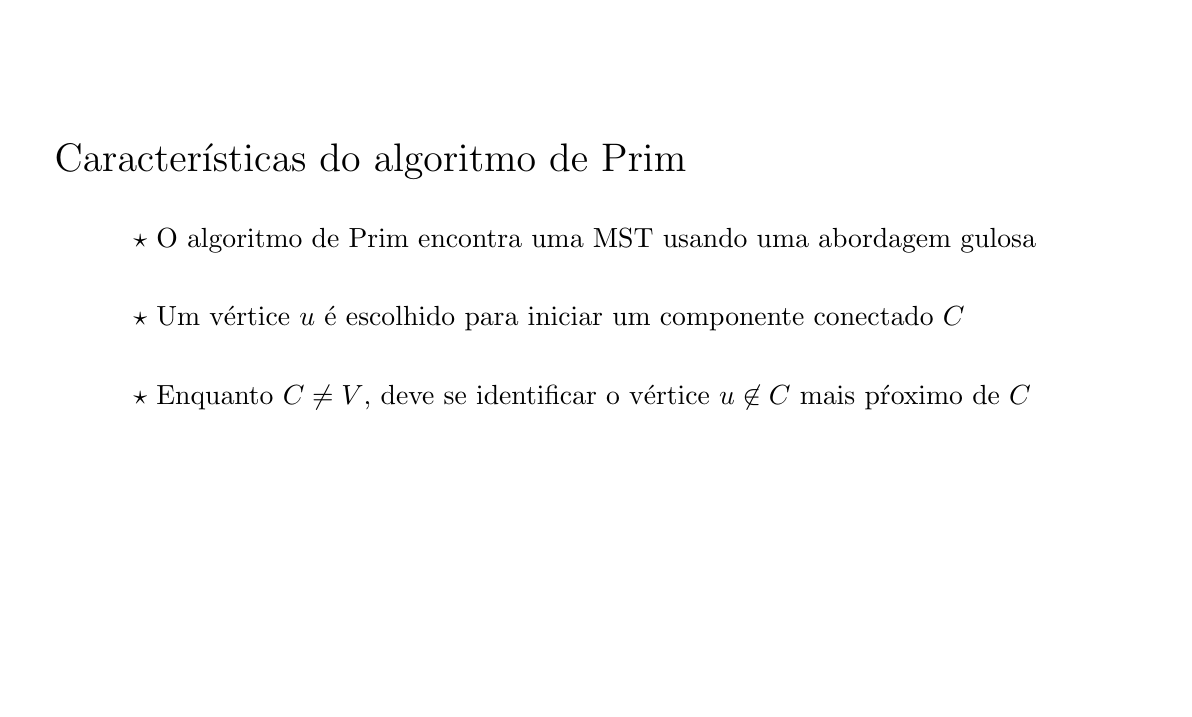
\begin{tikzpicture}
\node[draw,opacity=0] at (0, 0) {x};
\node[draw,opacity=0] at (14, 8) {x};

	\node[anchor=west] (title) at (0.0, 6.5) { \Large \bbbold{Características do algoritmo de Prim} };

	\node[anchor=west] (a) at (1.0, 5.5) { $\star$ \bbtext{O algoritmo de Prim encontra uma MST usando uma abordagem gulosa} };


	\node[anchor=west] (b) at (1.0, 4.5) { $\star$ \bbtext{Um vértice $u$ é escolhido para iniciar um componente conectado $C$} };


	\node[anchor=west] (c) at (1.0, 3.5) { $\star$ \bbtext{Enquanto $C \neq V$, deve se identificar o vértice $u\not\in C$ mais pŕoximo de $C$} };

\end{tikzpicture}
\end{frame}
\begin{frame}[plain,t]
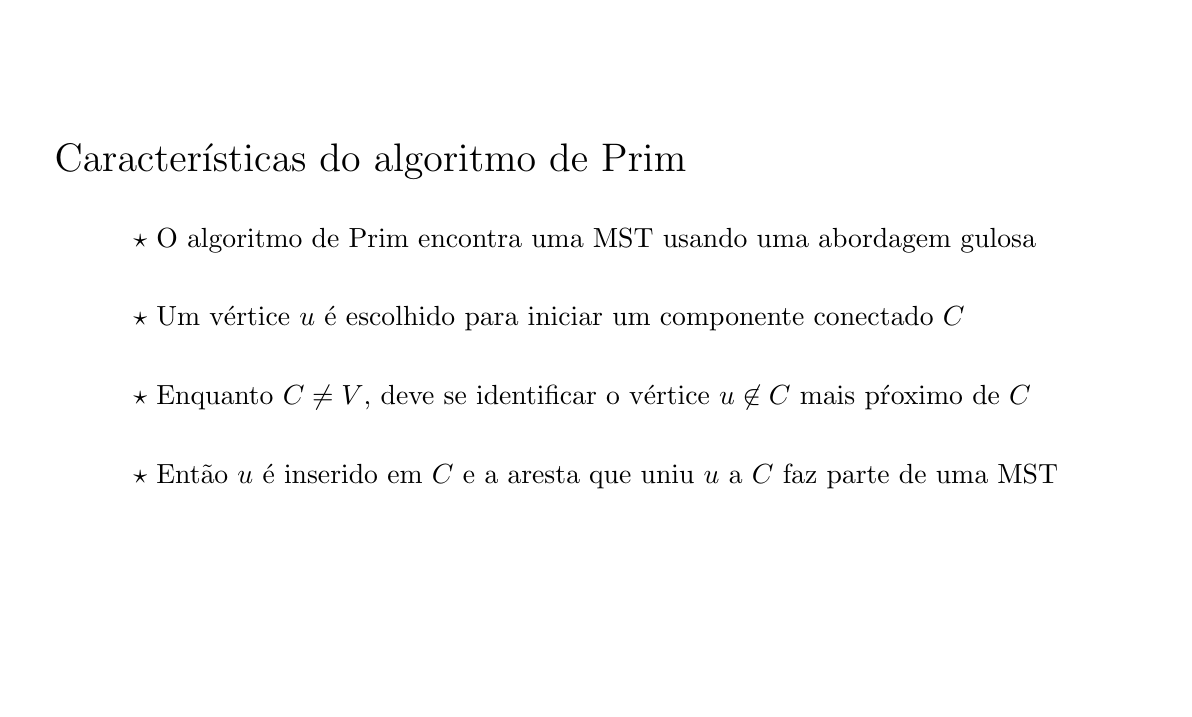
\begin{tikzpicture}
\node[draw,opacity=0] at (0, 0) {x};
\node[draw,opacity=0] at (14, 8) {x};

	\node[anchor=west] (title) at (0.0, 6.5) { \Large \bbbold{Características do algoritmo de Prim} };

	\node[anchor=west] (a) at (1.0, 5.5) { $\star$ \bbtext{O algoritmo de Prim encontra uma MST usando uma abordagem gulosa} };


	\node[anchor=west] (b) at (1.0, 4.5) { $\star$ \bbtext{Um vértice $u$ é escolhido para iniciar um componente conectado $C$} };


	\node[anchor=west] (c) at (1.0, 3.5) { $\star$ \bbtext{Enquanto $C \neq V$, deve se identificar o vértice $u\not\in C$ mais pŕoximo de $C$} };


	\node[anchor=west] (d) at (1.0, 2.5) { $\star$ \bbtext{Então $u$ é inserido em $C$ e a aresta que uniu $u$ a $C$ faz parte de uma MST} };

\end{tikzpicture}
\end{frame}
\begin{frame}[plain,t]
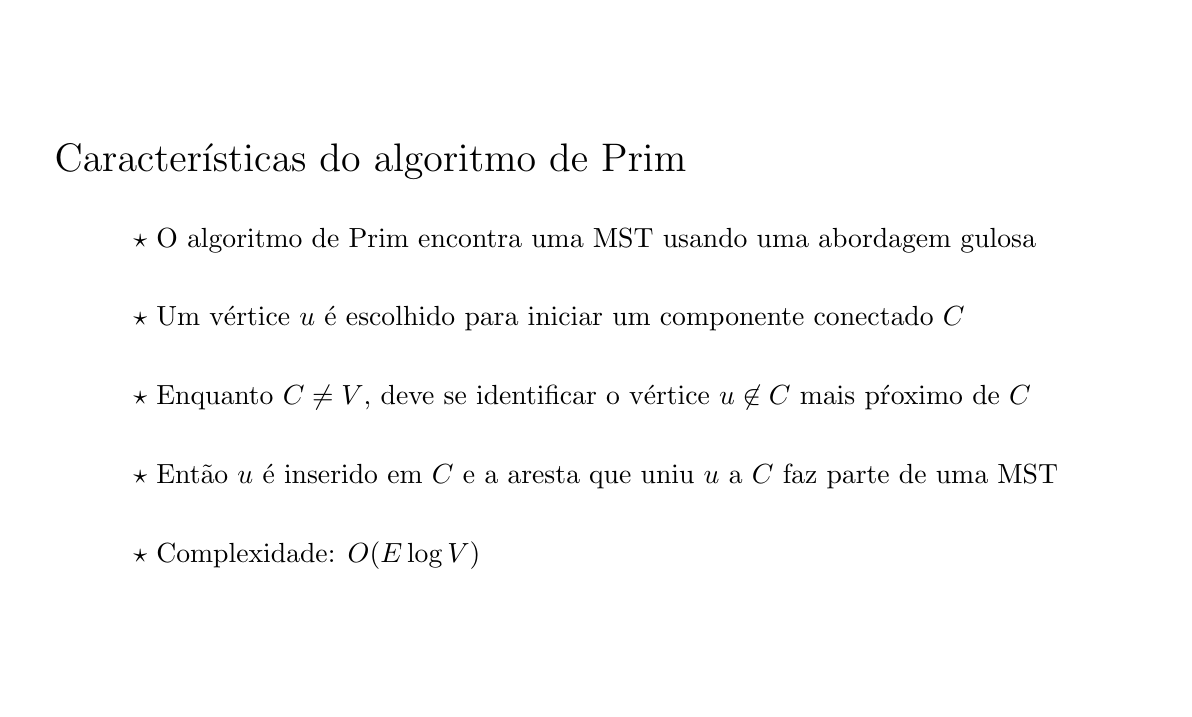
\begin{tikzpicture}
\node[draw,opacity=0] at (0, 0) {x};
\node[draw,opacity=0] at (14, 8) {x};

	\node[anchor=west] (title) at (0.0, 6.5) { \Large \bbbold{Características do algoritmo de Prim} };

	\node[anchor=west] (a) at (1.0, 5.5) { $\star$ \bbtext{O algoritmo de Prim encontra uma MST usando uma abordagem gulosa} };


	\node[anchor=west] (b) at (1.0, 4.5) { $\star$ \bbtext{Um vértice $u$ é escolhido para iniciar um componente conectado $C$} };


	\node[anchor=west] (c) at (1.0, 3.5) { $\star$ \bbtext{Enquanto $C \neq V$, deve se identificar o vértice $u\not\in C$ mais pŕoximo de $C$} };


	\node[anchor=west] (d) at (1.0, 2.5) { $\star$ \bbtext{Então $u$ é inserido em $C$ e a aresta que uniu $u$ a $C$ faz parte de uma MST} };


	\node[anchor=west] (e) at (1.0, 1.5) { $\star$ \bbtext{\bbbold{Complexidade}: $O(E\log V)$ } };

\end{tikzpicture}
\end{frame}
\begin{frame}[plain,t]
\begin{tikzpicture}
\node[draw,opacity=0] at (0, 0) {x};
\node[draw,opacity=0] at (14, 8) {x};

	\node[anchor=west] (title) at (0.0, 7.0) { \Large \bbbold{Pseudocódigo} };

\end{tikzpicture}
\end{frame}
\begin{frame}[plain,t]
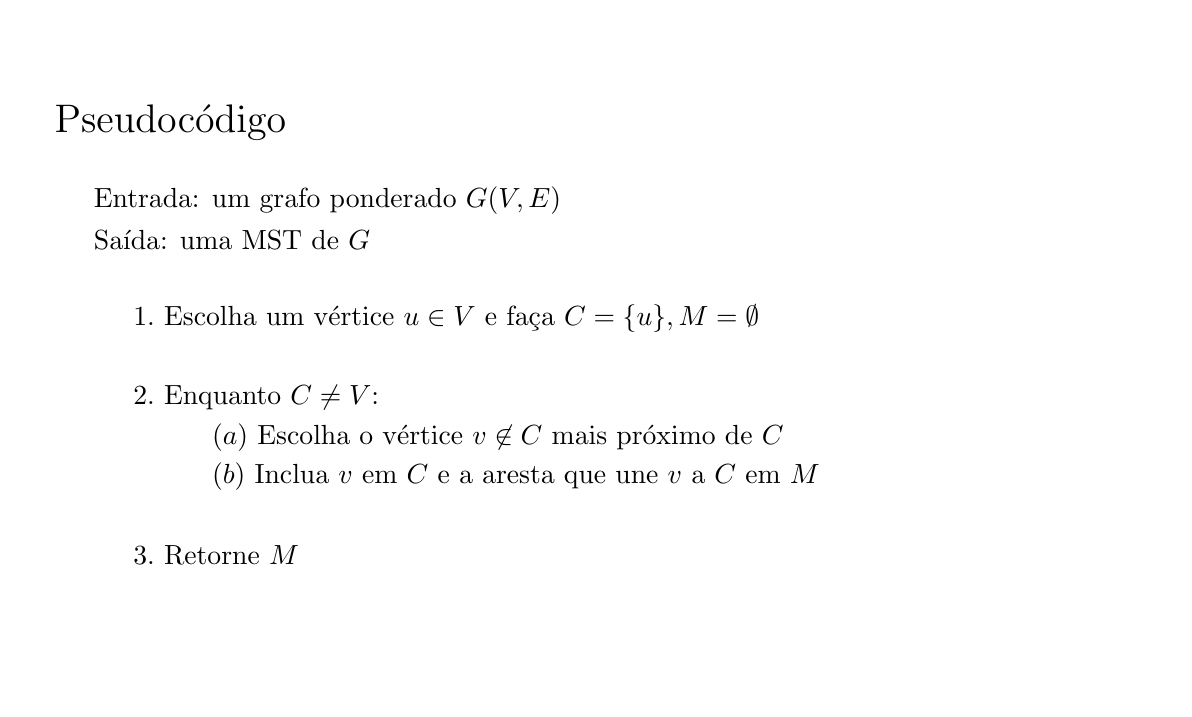
\begin{tikzpicture}
\node[draw,opacity=0] at (0, 0) {x};
\node[draw,opacity=0] at (14, 8) {x};

	\node[anchor=west] (title) at (0.0, 7.0) { \Large \bbbold{Pseudocódigo} };


	\node[anchor=west] (input) at (0.5, 6.0) { \bbemph{Entrada:} \bbtext{um grafo ponderado $G(V, E)$} };

	\node[anchor=west] (output) at (0.5, 5.5) { \bbemph{Saída:} \bbtext{uma MST de $G$} };

	\node[anchor=west] (step1) at (1.0, 4.5) { $1.$ \bbtext{Escolha um vértice $u\in V$ e faça $C = \{ u \}, M = \emptyset$} };

	\node[anchor=west] (step2) at (1.0, 3.5) { $2.$ \bbtext{Enquanto $C\neq V$:} };

	\node[anchor=west] (step2a) at (2.0, 3.0) { $(a)$ \bbtext{Escolha o vértice $v\not\in C$ mais próximo de $C$} };

	\node[anchor=west] (step2b) at (2.0, 2.5) { $(b)$ \bbtext{Inclua $v$ em $C$ e a aresta que une $v$ a $C$ em $M$} };

	\node[anchor=west] (step3) at (1.0, 1.5) { $3.$ \bbtext{Retorne $M$} };

\end{tikzpicture}
\end{frame}
\begin{frame}[plain,t]
\begin{tikzpicture}
\node[draw,opacity=0] at (0, 0) {x};
\node[draw,opacity=0] at (14, 8) {x};

	\node[very thick,draw,circle] (node1) at (10.0, 5.0) { \bbtext{1} };

	\node[very thick,draw,circle] (node2) at (7.0, 7.0) { \bbtext{2} };

	\node[very thick,draw,circle] (node3) at (4.0, 5.0) { \bbtext{3} };

	\node[very thick,draw,circle] (node4) at (10.0, 3.0) { \bbtext{4} };

	\node[very thick,draw,circle] (node5) at (7.0, 1.0) { \bbtext{5} };

	\node[very thick,draw,circle] (node6) at (4.0, 3.0) { \bbtext{6} };

	\draw[thick](node2) to node[above left] {\footnotesize \bbinfo{1}} (node3);

	\draw[thick](node4) to node[below right] {\footnotesize \bbinfo{1}} (node5);

	\draw[thick](node1) to node[right] {\footnotesize \bbinfo{2}} (node4);

	\draw[thick](node5) to node[above left,pos=0.3] {\footnotesize \bbinfo{2}} (node1);

	\draw[thick](node3) to node[above left] {\footnotesize \bbinfo{3}} (node4);

	\draw[thick](node1) to node[above right] {\footnotesize \bbinfo{4}} (node2);

	\draw[thick](node1) to node[above] {\footnotesize \bbinfo{5}} (node3);

	\draw[thick](node3) to node[left] {\footnotesize \bbinfo{7}} (node6);

	\draw[thick](node6) to node[above] {\footnotesize \bbinfo{8}} (node5);

\end{tikzpicture}
\end{frame}
\begin{frame}[plain,t]
\begin{tikzpicture}
\node[draw,opacity=0] at (0, 0) {x};
\node[draw,opacity=0] at (14, 8) {x};

	\node[very thick,draw,circle] (node1) at (10.0, 5.0) { \bbtext{1} };

	\node[very thick,draw,circle] (node2) at (7.0, 7.0) { \bbtext{2} };

	\node[very thick,draw,circle] (node3) at (4.0, 5.0) { \bbtext{3} };

	\node[very thick,draw,circle] (node4) at (10.0, 3.0) { \bbtext{4} };

	\node[very thick,draw,circle] (node5) at (7.0, 1.0) { \bbtext{5} };

	\node[very thick,draw,circle,fill=BBCyan] (node6) at (4.0, 3.0) { \bbtext{6} };

	\draw[thick](node2) to node[above left] {\footnotesize \bbinfo{1}} (node3);

	\draw[thick](node4) to node[below right] {\footnotesize \bbinfo{1}} (node5);

	\draw[thick](node1) to node[right] {\footnotesize \bbinfo{2}} (node4);

	\draw[thick](node5) to node[above left,pos=0.3] {\footnotesize \bbinfo{2}} (node1);

	\draw[thick](node3) to node[above left] {\footnotesize \bbinfo{3}} (node4);

	\draw[thick](node1) to node[above right] {\footnotesize \bbinfo{4}} (node2);

	\draw[thick](node1) to node[above] {\footnotesize \bbinfo{5}} (node3);

	\draw[thick](node3) to node[left] {\footnotesize \bbinfo{7}} (node6);

	\draw[thick](node6) to node[above] {\footnotesize \bbinfo{8}} (node5);



\end{tikzpicture}
\end{frame}
\begin{frame}[plain,t]
\begin{tikzpicture}
\node[draw,opacity=0] at (0, 0) {x};
\node[draw,opacity=0] at (14, 8) {x};

	\node[very thick,draw,circle] (node1) at (10.0, 5.0) { \bbtext{1} };

	\node[very thick,draw,circle] (node2) at (7.0, 7.0) { \bbtext{2} };

	\node[very thick,draw,circle,fill=BBCyan] (node3) at (4.0, 5.0) { \bbtext{3} };

	\node[very thick,draw,circle] (node4) at (10.0, 3.0) { \bbtext{4} };

	\node[very thick,draw,circle] (node5) at (7.0, 1.0) { \bbtext{5} };

	\node[very thick,draw,circle,fill=BBCyan] (node6) at (4.0, 3.0) { \bbtext{6} };

	\draw[thick](node2) to node[above left] {\footnotesize \bbinfo{1}} (node3);

	\draw[thick](node4) to node[below right] {\footnotesize \bbinfo{1}} (node5);

	\draw[thick](node1) to node[right] {\footnotesize \bbinfo{2}} (node4);

	\draw[thick](node5) to node[above left,pos=0.3] {\footnotesize \bbinfo{2}} (node1);

	\draw[thick](node3) to node[above left] {\footnotesize \bbinfo{3}} (node4);

	\draw[thick](node1) to node[above right] {\footnotesize \bbinfo{4}} (node2);

	\draw[thick](node1) to node[above] {\footnotesize \bbinfo{5}} (node3);

	\draw[thick,very thick,dashed,color=BBGreen](node3) to node[left] {\footnotesize \bbinfo{7}} (node6);

	\draw[thick](node6) to node[above] {\footnotesize \bbinfo{8}} (node5);






\end{tikzpicture}
\end{frame}
\begin{frame}[plain,t]
\begin{tikzpicture}
\node[draw,opacity=0] at (0, 0) {x};
\node[draw,opacity=0] at (14, 8) {x};

	\node[very thick,draw,circle] (node1) at (10.0, 5.0) { \bbtext{1} };

	\node[very thick,draw,circle,fill=BBCyan] (node2) at (7.0, 7.0) { \bbtext{2} };

	\node[very thick,draw,circle,fill=BBCyan] (node3) at (4.0, 5.0) { \bbtext{3} };

	\node[very thick,draw,circle] (node4) at (10.0, 3.0) { \bbtext{4} };

	\node[very thick,draw,circle] (node5) at (7.0, 1.0) { \bbtext{5} };

	\node[very thick,draw,circle,fill=BBCyan] (node6) at (4.0, 3.0) { \bbtext{6} };

	\draw[thick,very thick,dashed,color=BBGreen](node2) to node[above left] {\footnotesize \bbinfo{1}} (node3);

	\draw[thick](node4) to node[below right] {\footnotesize \bbinfo{1}} (node5);

	\draw[thick](node1) to node[right] {\footnotesize \bbinfo{2}} (node4);

	\draw[thick](node5) to node[above left,pos=0.3] {\footnotesize \bbinfo{2}} (node1);

	\draw[thick](node3) to node[above left] {\footnotesize \bbinfo{3}} (node4);

	\draw[thick](node1) to node[above right] {\footnotesize \bbinfo{4}} (node2);

	\draw[thick](node1) to node[above] {\footnotesize \bbinfo{5}} (node3);

	\draw[thick,very thick,dashed,color=BBGreen](node3) to node[left] {\footnotesize \bbinfo{7}} (node6);

	\draw[thick](node6) to node[above] {\footnotesize \bbinfo{8}} (node5);









\end{tikzpicture}
\end{frame}
\begin{frame}[plain,t]
\begin{tikzpicture}
\node[draw,opacity=0] at (0, 0) {x};
\node[draw,opacity=0] at (14, 8) {x};

	\node[very thick,draw,circle] (node1) at (10.0, 5.0) { \bbtext{1} };

	\node[very thick,draw,circle,fill=BBCyan] (node2) at (7.0, 7.0) { \bbtext{2} };

	\node[very thick,draw,circle,fill=BBCyan] (node3) at (4.0, 5.0) { \bbtext{3} };

	\node[very thick,draw,circle,fill=BBCyan] (node4) at (10.0, 3.0) { \bbtext{4} };

	\node[very thick,draw,circle] (node5) at (7.0, 1.0) { \bbtext{5} };

	\node[very thick,draw,circle,fill=BBCyan] (node6) at (4.0, 3.0) { \bbtext{6} };

	\draw[thick,very thick,dashed,color=BBGreen](node2) to node[above left] {\footnotesize \bbinfo{1}} (node3);

	\draw[thick](node4) to node[below right] {\footnotesize \bbinfo{1}} (node5);

	\draw[thick](node1) to node[right] {\footnotesize \bbinfo{2}} (node4);

	\draw[thick](node5) to node[above left,pos=0.3] {\footnotesize \bbinfo{2}} (node1);

	\draw[thick,very thick,dashed,color=BBGreen](node3) to node[above left] {\footnotesize \bbinfo{3}} (node4);

	\draw[thick](node1) to node[above right] {\footnotesize \bbinfo{4}} (node2);

	\draw[thick](node1) to node[above] {\footnotesize \bbinfo{5}} (node3);

	\draw[thick,very thick,dashed,color=BBGreen](node3) to node[left] {\footnotesize \bbinfo{7}} (node6);

	\draw[thick](node6) to node[above] {\footnotesize \bbinfo{8}} (node5);












\end{tikzpicture}
\end{frame}
\begin{frame}[plain,t]
\begin{tikzpicture}
\node[draw,opacity=0] at (0, 0) {x};
\node[draw,opacity=0] at (14, 8) {x};

	\node[very thick,draw,circle] (node1) at (10.0, 5.0) { \bbtext{1} };

	\node[very thick,draw,circle,fill=BBCyan] (node2) at (7.0, 7.0) { \bbtext{2} };

	\node[very thick,draw,circle,fill=BBCyan] (node3) at (4.0, 5.0) { \bbtext{3} };

	\node[very thick,draw,circle,fill=BBCyan] (node4) at (10.0, 3.0) { \bbtext{4} };

	\node[very thick,draw,circle,fill=BBCyan] (node5) at (7.0, 1.0) { \bbtext{5} };

	\node[very thick,draw,circle,fill=BBCyan] (node6) at (4.0, 3.0) { \bbtext{6} };

	\draw[thick,very thick,dashed,color=BBGreen](node2) to node[above left] {\footnotesize \bbinfo{1}} (node3);

	\draw[thick,very thick,dashed,color=BBGreen](node4) to node[below right] {\footnotesize \bbinfo{1}} (node5);

	\draw[thick](node1) to node[right] {\footnotesize \bbinfo{2}} (node4);

	\draw[thick](node5) to node[above left,pos=0.3] {\footnotesize \bbinfo{2}} (node1);

	\draw[thick,very thick,dashed,color=BBGreen](node3) to node[above left] {\footnotesize \bbinfo{3}} (node4);

	\draw[thick](node1) to node[above right] {\footnotesize \bbinfo{4}} (node2);

	\draw[thick](node1) to node[above] {\footnotesize \bbinfo{5}} (node3);

	\draw[thick,very thick,dashed,color=BBGreen](node3) to node[left] {\footnotesize \bbinfo{7}} (node6);

	\draw[thick](node6) to node[above] {\footnotesize \bbinfo{8}} (node5);















\end{tikzpicture}
\end{frame}
\begin{frame}[plain,t]
\begin{tikzpicture}
\node[draw,opacity=0] at (0, 0) {x};
\node[draw,opacity=0] at (14, 8) {x};

	\node[very thick,draw,circle,fill=BBCyan] (node1) at (10.0, 5.0) { \bbtext{1} };

	\node[very thick,draw,circle,fill=BBCyan] (node2) at (7.0, 7.0) { \bbtext{2} };

	\node[very thick,draw,circle,fill=BBCyan] (node3) at (4.0, 5.0) { \bbtext{3} };

	\node[very thick,draw,circle,fill=BBCyan] (node4) at (10.0, 3.0) { \bbtext{4} };

	\node[very thick,draw,circle,fill=BBCyan] (node5) at (7.0, 1.0) { \bbtext{5} };

	\node[very thick,draw,circle,fill=BBCyan] (node6) at (4.0, 3.0) { \bbtext{6} };

	\draw[thick,very thick,dashed,color=BBGreen](node2) to node[above left] {\footnotesize \bbinfo{1}} (node3);

	\draw[thick,very thick,dashed,color=BBGreen](node4) to node[below right] {\footnotesize \bbinfo{1}} (node5);

	\draw[thick,very thick,dashed,color=BBGreen](node1) to node[right] {\footnotesize \bbinfo{2}} (node4);

	\draw[thick](node5) to node[above left,pos=0.3] {\footnotesize \bbinfo{2}} (node1);

	\draw[thick,very thick,dashed,color=BBGreen](node3) to node[above left] {\footnotesize \bbinfo{3}} (node4);

	\draw[thick](node1) to node[above right] {\footnotesize \bbinfo{4}} (node2);

	\draw[thick](node1) to node[above] {\footnotesize \bbinfo{5}} (node3);

	\draw[thick,very thick,dashed,color=BBGreen](node3) to node[left] {\footnotesize \bbinfo{7}} (node6);

	\draw[thick](node6) to node[above] {\footnotesize \bbinfo{8}} (node5);


















\end{tikzpicture}
\end{frame}
\begin{frame}[plain,t]
\begin{tikzpicture}
\node[draw,opacity=0] at (0, 0) {x};
\node[draw,opacity=0] at (14, 8) {x};

	\node[anchor=west] (title) at (0.0, 6.5) { \Large \bbbold{Identificação eficiente do vértice mais próximo de $C$} };

\end{tikzpicture}
\end{frame}
\begin{frame}[plain,t]
\begin{tikzpicture}
\node[draw,opacity=0] at (0, 0) {x};
\node[draw,opacity=0] at (14, 8) {x};

	\node[anchor=west] (title) at (0.0, 6.5) { \Large \bbbold{Identificação eficiente do vértice mais próximo de $C$} };


	\node[anchor=west] (a) at (1.0, 5.5) { $\star$ \bbtext{A complexidade do algoritmo de Prim depende da identificação eficiente do} };

	\node[anchor=west] (a1) at (0.5, 5.0) { \bbtext{vértice $v$ mais próximo de $C$} };

\end{tikzpicture}
\end{frame}
\begin{frame}[plain,t]
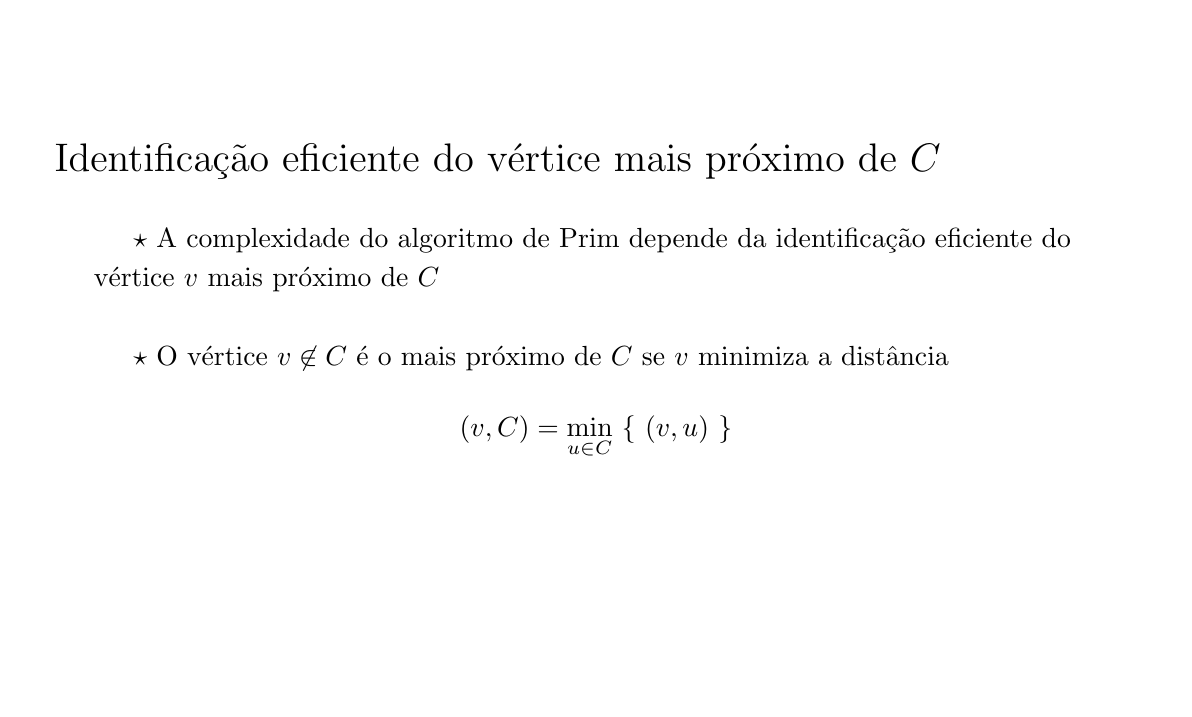
\begin{tikzpicture}
\node[draw,opacity=0] at (0, 0) {x};
\node[draw,opacity=0] at (14, 8) {x};

	\node[anchor=west] (title) at (0.0, 6.5) { \Large \bbbold{Identificação eficiente do vértice mais próximo de $C$} };


	\node[anchor=west] (a) at (1.0, 5.5) { $\star$ \bbtext{A complexidade do algoritmo de Prim depende da identificação eficiente do} };

	\node[anchor=west] (a1) at (0.5, 5.0) { \bbtext{vértice $v$ mais próximo de $C$} };


	\node[anchor=west] (b) at (1.0, 4.0) { $\star$ \bbtext{O vértice $v\not\in C$ é o mais próximo de $C$ se $v$ minimiza a distância} };

	\node[] (b1) at (7.0, 3.0) { $\displaystyle \dist(v, C) = \min_{u\in C}\ \{\ \dist(v, u)\ \}$ };

\end{tikzpicture}
\end{frame}
\begin{frame}[plain,t]
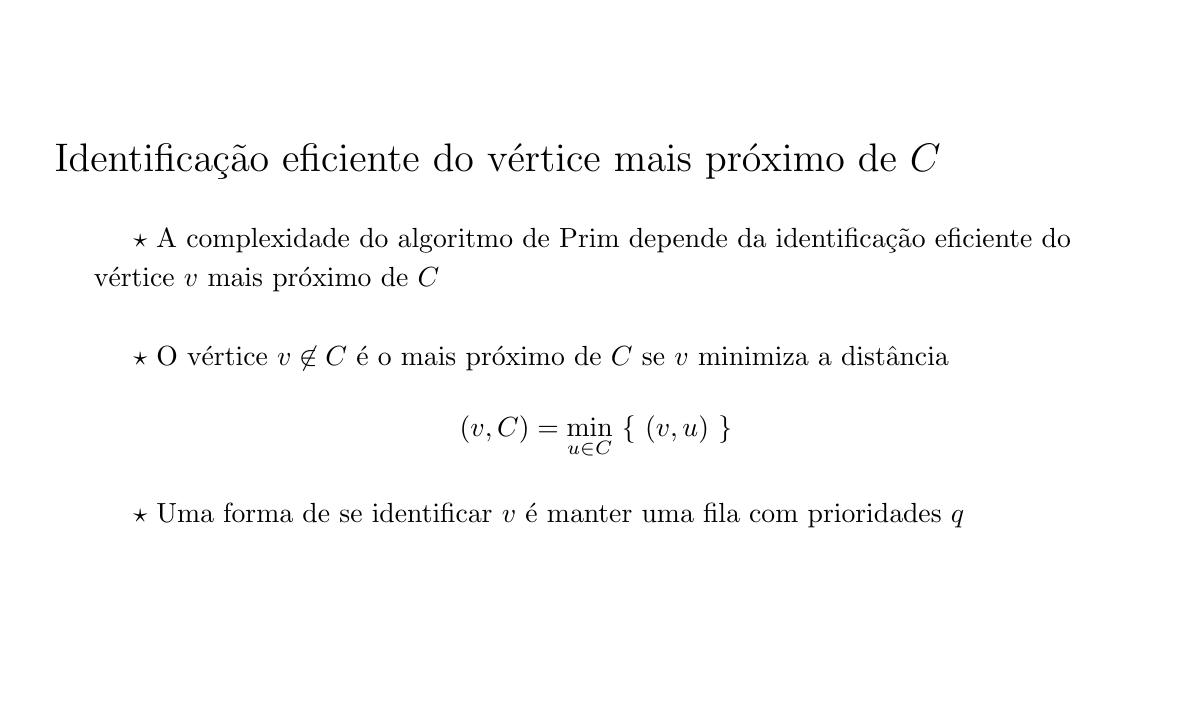
\begin{tikzpicture}
\node[draw,opacity=0] at (0, 0) {x};
\node[draw,opacity=0] at (14, 8) {x};

	\node[anchor=west] (title) at (0.0, 6.5) { \Large \bbbold{Identificação eficiente do vértice mais próximo de $C$} };


	\node[anchor=west] (a) at (1.0, 5.5) { $\star$ \bbtext{A complexidade do algoritmo de Prim depende da identificação eficiente do} };

	\node[anchor=west] (a1) at (0.5, 5.0) { \bbtext{vértice $v$ mais próximo de $C$} };


	\node[anchor=west] (b) at (1.0, 4.0) { $\star$ \bbtext{O vértice $v\not\in C$ é o mais próximo de $C$ se $v$ minimiza a distância} };

	\node[] (b1) at (7.0, 3.0) { $\displaystyle \dist(v, C) = \min_{u\in C}\ \{\ \dist(v, u)\ \}$ };


	\node[anchor=west] (c) at (1.0, 2.0) { $\star$ \bbtext{Uma forma de se identificar $v$ é manter uma fila com prioridades $q$} };

\end{tikzpicture}
\end{frame}
\begin{frame}[plain,t]
\begin{tikzpicture}
\node[draw,opacity=0] at (0, 0) {x};
\node[draw,opacity=0] at (14, 8) {x};

	\node[anchor=west] (title) at (0.0, 6.5) { \Large \bbbold{Identificação eficiente do vértice mais próximo de $C$} };

	\node[anchor=west] (a) at (1.0, 5.5) { $\star$ \bbtext{Inicialmente, $q$ estará vazia} };

\end{tikzpicture}
\end{frame}
\begin{frame}[plain,t]
\begin{tikzpicture}
\node[draw,opacity=0] at (0, 0) {x};
\node[draw,opacity=0] at (14, 8) {x};

	\node[anchor=west] (title) at (0.0, 6.5) { \Large \bbbold{Identificação eficiente do vértice mais próximo de $C$} };

	\node[anchor=west] (a) at (1.0, 5.5) { $\star$ \bbtext{Inicialmente, $q$ estará vazia} };


	\node[anchor=west] (b) at (1.0, 4.5) { $\star$ \bbtext{Esta fila será ordenada, de forma ascendente, pelas distâncias até $C$} };


\end{tikzpicture}
\end{frame}
\begin{frame}[plain,t]
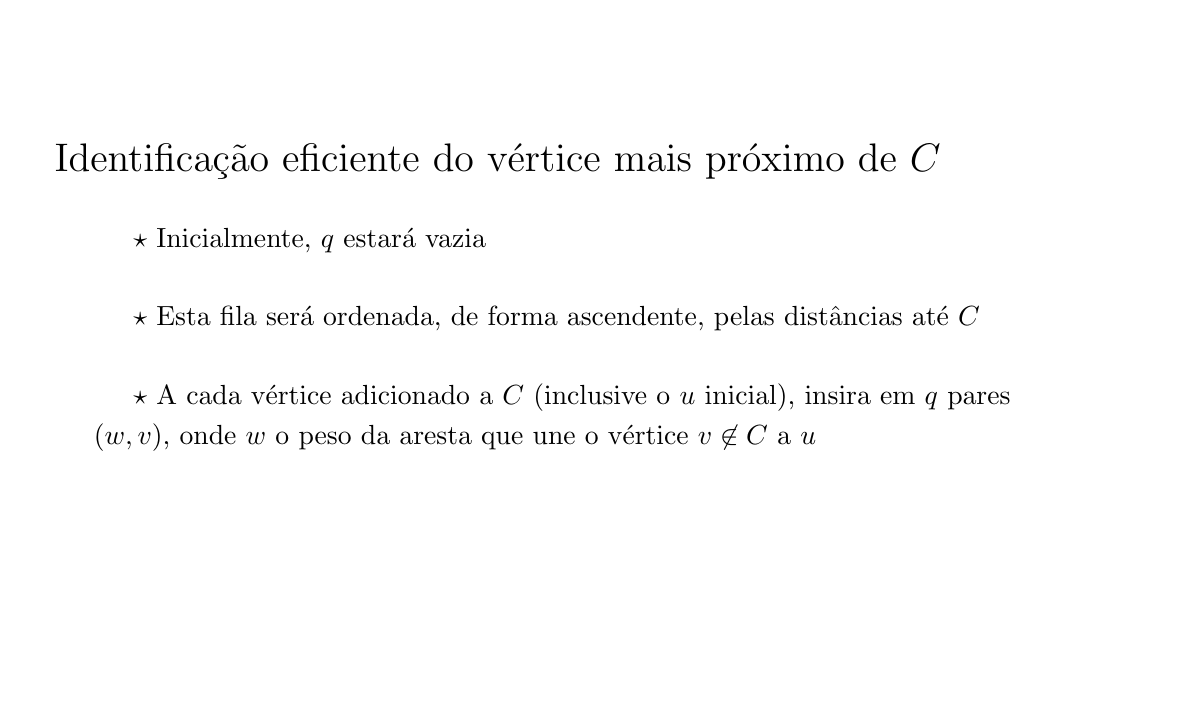
\begin{tikzpicture}
\node[draw,opacity=0] at (0, 0) {x};
\node[draw,opacity=0] at (14, 8) {x};

	\node[anchor=west] (title) at (0.0, 6.5) { \Large \bbbold{Identificação eficiente do vértice mais próximo de $C$} };

	\node[anchor=west] (a) at (1.0, 5.5) { $\star$ \bbtext{Inicialmente, $q$ estará vazia} };


	\node[anchor=west] (b) at (1.0, 4.5) { $\star$ \bbtext{Esta fila será ordenada, de forma ascendente, pelas distâncias até $C$} };



	\node[anchor=west] (c) at (1.0, 3.5) { $\star$ \bbtext{A cada vértice adicionado a $C$ (inclusive o $u$ inicial), insira em $q$ pares} };

	\node[anchor=west] (c1) at (0.5, 3.0) { \bbtext{$(w, v)$, onde $w$ o peso da aresta que une o vértice $v\not\in C$ a $u$} };

\end{tikzpicture}
\end{frame}
\begin{frame}[plain,t]
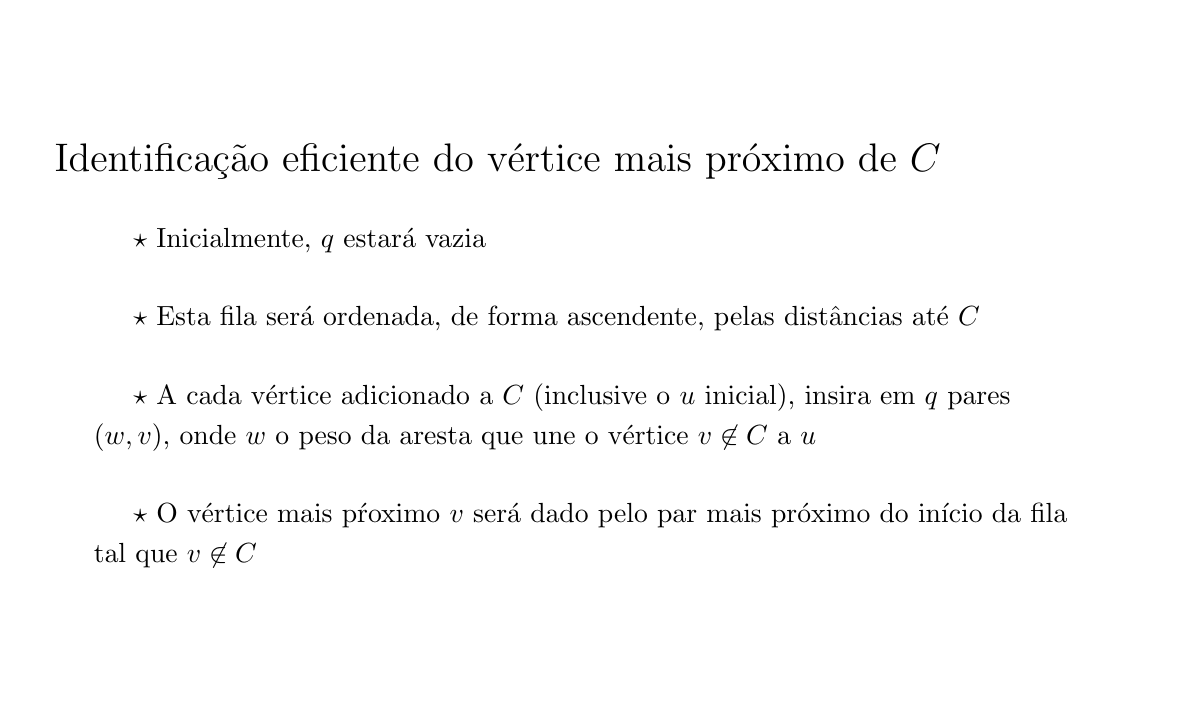
\begin{tikzpicture}
\node[draw,opacity=0] at (0, 0) {x};
\node[draw,opacity=0] at (14, 8) {x};

	\node[anchor=west] (title) at (0.0, 6.5) { \Large \bbbold{Identificação eficiente do vértice mais próximo de $C$} };

	\node[anchor=west] (a) at (1.0, 5.5) { $\star$ \bbtext{Inicialmente, $q$ estará vazia} };


	\node[anchor=west] (b) at (1.0, 4.5) { $\star$ \bbtext{Esta fila será ordenada, de forma ascendente, pelas distâncias até $C$} };



	\node[anchor=west] (c) at (1.0, 3.5) { $\star$ \bbtext{A cada vértice adicionado a $C$ (inclusive o $u$ inicial), insira em $q$ pares} };

	\node[anchor=west] (c1) at (0.5, 3.0) { \bbtext{$(w, v)$, onde $w$ o peso da aresta que une o vértice $v\not\in C$ a $u$} };


	\node[anchor=west] (d) at (1.0, 2.0) { $\star$ \bbtext{O vértice mais pŕoximo $v$ será dado pelo par mais próximo do início da fila} };

	\node[anchor=west] (d1) at (0.5, 1.5) { \bbtext{tal que $v\not\in C$} };


\end{tikzpicture}
\end{frame}
\begin{frame}[plain,t]

\inputsnippet{cpp}{11}{26}{codes/prim.cpp}

\end{frame}
\begin{frame}[plain,t]

\inputsnippet{cpp}{27}{40}{codes/prim.cpp}

\end{frame}
\begin{frame}[plain,t]
\begin{tikzpicture}
\node[draw,opacity=0] at (0, 0) {x};
\node[draw,opacity=0] at (14, 8) {x};

	\node[anchor=west] (title) at (0.0, 6.5) { \Large \bbbold{Aplicação: Minimax} };

\end{tikzpicture}
\end{frame}
\begin{frame}[plain,t]
\begin{tikzpicture}
\node[draw,opacity=0] at (0, 0) {x};
\node[draw,opacity=0] at (14, 8) {x};

	\node[anchor=west] (title) at (0.0, 6.5) { \Large \bbbold{Aplicação: Minimax} };


	\node[anchor=west] (a) at (1.0, 5.5) { $\star$ \bbtext{Uma MST minimiza o maior peso entre as arestas presente em qualquer } };

	\node[anchor=west] (a1) at (0.5, 5.0) { \bbtext{árvore geradora} };

\end{tikzpicture}
\end{frame}
\begin{frame}[plain,t]
\begin{tikzpicture}
\node[draw,opacity=0] at (0, 0) {x};
\node[draw,opacity=0] at (14, 8) {x};

	\node[anchor=west] (title) at (0.0, 6.5) { \Large \bbbold{Aplicação: Minimax} };


	\node[anchor=west] (a) at (1.0, 5.5) { $\star$ \bbtext{Uma MST minimiza o maior peso entre as arestas presente em qualquer } };

	\node[anchor=west] (a1) at (0.5, 5.0) { \bbtext{árvore geradora} };


	\node[anchor=west] (b) at (1.0, 4.0) { $\star$ \bbtext{O problema de se minimizar tal peso é denominado \bbenglish{minimax}} };

\end{tikzpicture}
\end{frame}
\begin{frame}[plain,t]
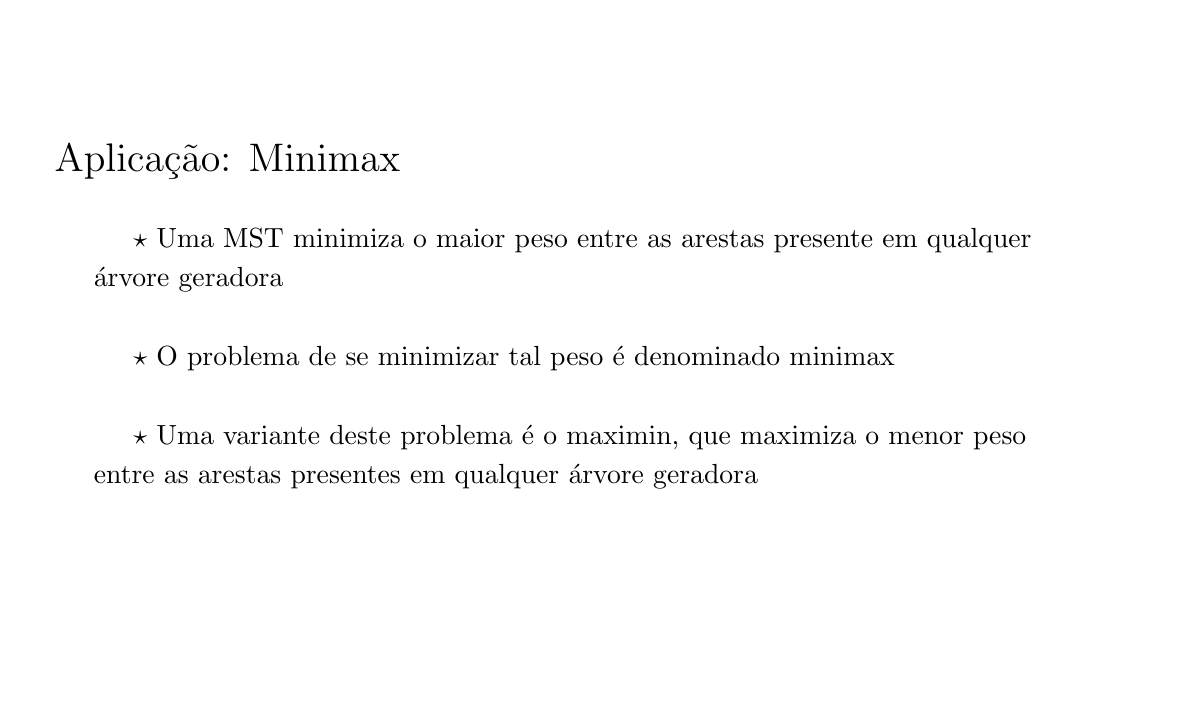
\begin{tikzpicture}
\node[draw,opacity=0] at (0, 0) {x};
\node[draw,opacity=0] at (14, 8) {x};

	\node[anchor=west] (title) at (0.0, 6.5) { \Large \bbbold{Aplicação: Minimax} };


	\node[anchor=west] (a) at (1.0, 5.5) { $\star$ \bbtext{Uma MST minimiza o maior peso entre as arestas presente em qualquer } };

	\node[anchor=west] (a1) at (0.5, 5.0) { \bbtext{árvore geradora} };


	\node[anchor=west] (b) at (1.0, 4.0) { $\star$ \bbtext{O problema de se minimizar tal peso é denominado \bbenglish{minimax}} };


	\node[anchor=west] (c) at (1.0, 3.0) { $\star$ \bbtext{Uma variante deste problema é o \bbenglish{maximin}, que maximiza o menor peso} };

	\node[anchor=west] (c1) at (0.5, 2.5) { \bbtext{entre as arestas presentes em qualquer árvore geradora} };

\end{tikzpicture}
\end{frame}
\begin{frame}[plain,t]
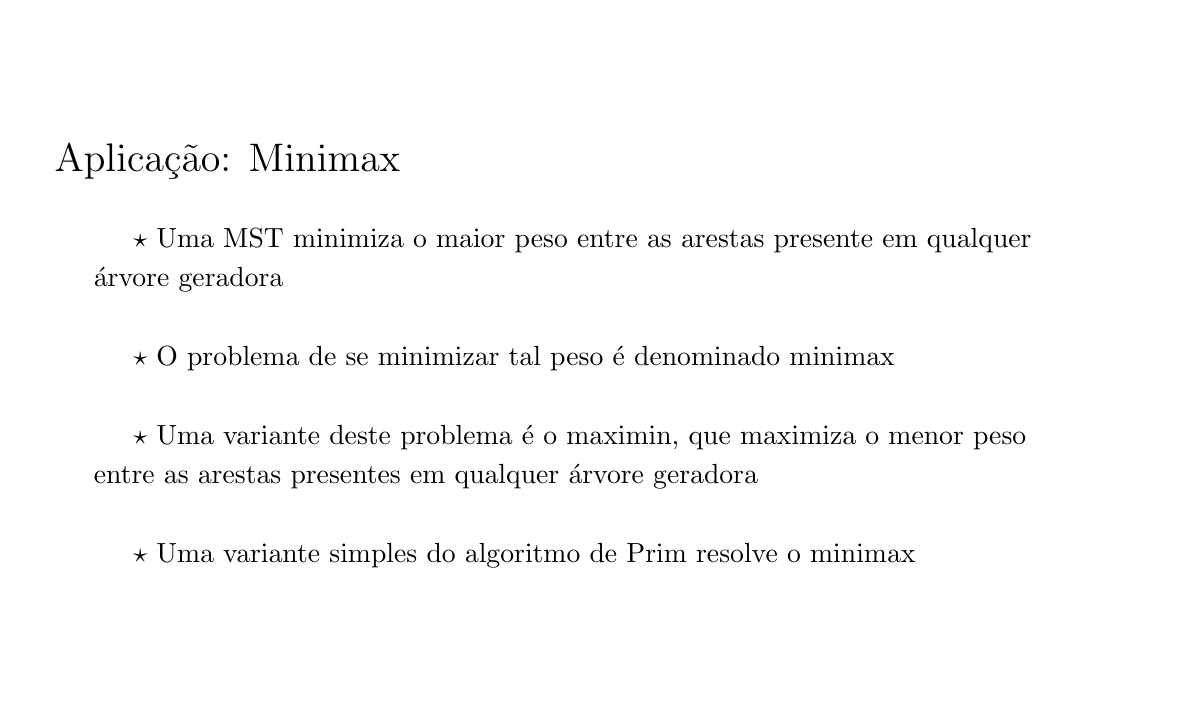
\begin{tikzpicture}
\node[draw,opacity=0] at (0, 0) {x};
\node[draw,opacity=0] at (14, 8) {x};

	\node[anchor=west] (title) at (0.0, 6.5) { \Large \bbbold{Aplicação: Minimax} };


	\node[anchor=west] (a) at (1.0, 5.5) { $\star$ \bbtext{Uma MST minimiza o maior peso entre as arestas presente em qualquer } };

	\node[anchor=west] (a1) at (0.5, 5.0) { \bbtext{árvore geradora} };


	\node[anchor=west] (b) at (1.0, 4.0) { $\star$ \bbtext{O problema de se minimizar tal peso é denominado \bbenglish{minimax}} };


	\node[anchor=west] (c) at (1.0, 3.0) { $\star$ \bbtext{Uma variante deste problema é o \bbenglish{maximin}, que maximiza o menor peso} };

	\node[anchor=west] (c1) at (0.5, 2.5) { \bbtext{entre as arestas presentes em qualquer árvore geradora} };


	\node[anchor=west] (d) at (1.0, 1.5) { $\star$ \bbtext{Uma variante simples do algoritmo de Prim resolve o \bbenglish{minimax}} };


\end{tikzpicture}
\end{frame}
\begin{frame}[plain,t]
\begin{tikzpicture}
\node[draw,opacity=0] at (0, 0) {x};
\node[draw,opacity=0] at (14, 8) {x};

	\node[very thick,draw,circle] (node1) at (10.0, 5.0) { \bbtext{1} };

	\node[very thick,draw,circle] (node2) at (7.0, 7.0) { \bbtext{2} };

	\node[very thick,draw,circle] (node3) at (4.0, 5.0) { \bbtext{3} };

	\node[very thick,draw,circle] (node4) at (10.0, 3.0) { \bbtext{4} };

	\node[very thick,draw,circle] (node5) at (7.0, 1.0) { \bbtext{5} };

	\node[very thick,draw,circle] (node6) at (4.0, 3.0) { \bbtext{6} };

	\draw[thick](node2) to node[above left] {\footnotesize \bbinfo{1}} (node3);

	\draw[thick](node4) to node[below right] {\footnotesize \bbinfo{1}} (node5);

	\draw[thick](node1) to node[right] {\footnotesize \bbinfo{2}} (node4);

	\draw[thick](node5) to node[above left,pos=0.3] {\footnotesize \bbinfo{2}} (node1);

	\draw[thick](node3) to node[above left] {\footnotesize \bbinfo{3}} (node4);

	\draw[thick](node1) to node[above right] {\footnotesize \bbinfo{4}} (node2);

	\draw[thick](node1) to node[above] {\footnotesize \bbinfo{5}} (node3);

	\draw[thick](node3) to node[right] {\footnotesize \bbinfo{7}} (node6);

	\draw[thick](node6) to node[above] {\footnotesize \bbinfo{8}} (node5);

\end{tikzpicture}
\end{frame}
\begin{frame}[plain,t]
\begin{tikzpicture}
\node[draw,opacity=0] at (0, 0) {x};
\node[draw,opacity=0] at (14, 8) {x};

	\node[very thick,draw,circle] (node1) at (10.0, 5.0) { \bbtext{1} };

	\node[very thick,draw,circle] (node2) at (7.0, 7.0) { \bbtext{2} };

	\node[very thick,draw,circle] (node3) at (4.0, 5.0) { \bbtext{3} };

	\node[very thick,draw,circle] (node4) at (10.0, 3.0) { \bbtext{4} };

	\node[very thick,draw,circle] (node5) at (7.0, 1.0) { \bbtext{5} };

	\node[very thick,draw,circle] (node6) at (4.0, 3.0) { \bbtext{6} };

	\draw[thick,very thick,dashed,color=BBGreen](node2) to node[above left] {\footnotesize \bbinfo{1}} (node3);

	\draw[thick,very thick,dashed,color=BBGreen](node4) to node[below right] {\footnotesize \bbinfo{1}} (node5);

	\draw[thick,very thick,dashed,color=BBGreen](node1) to node[right] {\footnotesize \bbinfo{2}} (node4);

	\draw[thick](node5) to node[above left,pos=0.3] {\footnotesize \bbinfo{2}} (node1);

	\draw[thick,very thick,dashed,color=BBGreen](node3) to node[above left] {\footnotesize \bbinfo{3}} (node4);

	\draw[thick](node1) to node[above right] {\footnotesize \bbinfo{4}} (node2);

	\draw[thick](node1) to node[above] {\footnotesize \bbinfo{5}} (node3);

	\draw[thick,very thick,color=BBGreen](node3) to node[right] {\footnotesize \bbinfo{7}} (node6);

	\draw[thick](node6) to node[above] {\footnotesize \bbinfo{8}} (node5);







	\node[anchor=east] (r) at (3.0, 4.0) { \footnotesize \bbcomment{minimax} };

	\draw[color=BBViolet,-latex] (3.05, 4.0) to  (3.85, 4.0);

\end{tikzpicture}
\end{frame}
\begin{frame}[plain,t]

\inputsnippet{cpp}{11}{26}{codes/minimax.cpp}

\end{frame}
\begin{frame}[plain,t]

\inputsnippet{cpp}{27}{40}{codes/minimax.cpp}

\end{frame}
\begin{frame}[plain,t]
\begin{tikzpicture}
\node[draw,opacity=0] at (0, 0) {x};
\node[draw,opacity=0] at (14, 8) {x};

	\node[anchor=west] (title) at (0.0, 7.0) { \Large \bbbold{Aplicação: Menor Subgrafo Gerador} };

\end{tikzpicture}
\end{frame}
\begin{frame}[plain,t]
\begin{tikzpicture}
\node[draw,opacity=0] at (0, 0) {x};
\node[draw,opacity=0] at (14, 8) {x};

	\node[anchor=west] (title) at (0.0, 7.0) { \Large \bbbold{Aplicação: Menor Subgrafo Gerador} };


	\node[anchor=west] (a) at (1.0, 6.0) { $\star$ \bbtext{Seja $G(V, E)$ um grafo conectado e ponderado e $E'\subset E$} };

\end{tikzpicture}
\end{frame}
\begin{frame}[plain,t]
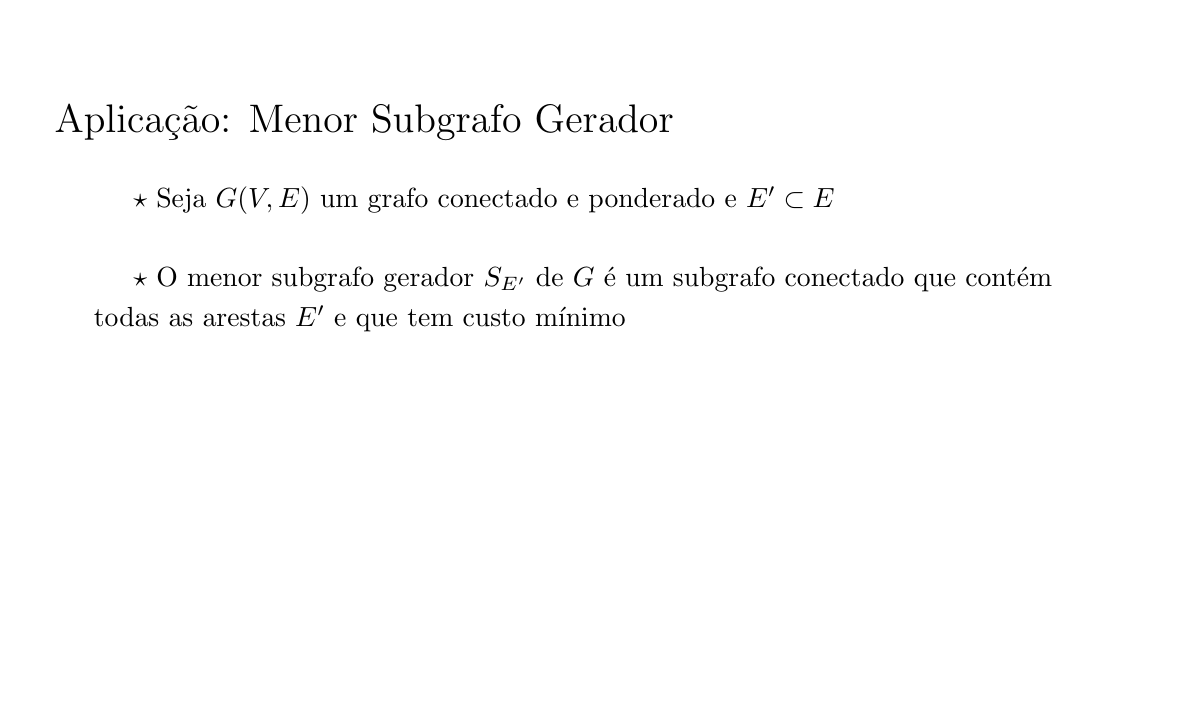
\begin{tikzpicture}
\node[draw,opacity=0] at (0, 0) {x};
\node[draw,opacity=0] at (14, 8) {x};

	\node[anchor=west] (title) at (0.0, 7.0) { \Large \bbbold{Aplicação: Menor Subgrafo Gerador} };


	\node[anchor=west] (a) at (1.0, 6.0) { $\star$ \bbtext{Seja $G(V, E)$ um grafo conectado e ponderado e $E'\subset E$} };


	\node[anchor=west] (b) at (1.0, 5.0) { $\star$ \bbtext{O menor subgrafo gerador $S_{E'}$ de $G$ é um subgrafo conectado que contém} };

	\node[anchor=west] (b1) at (0.5, 4.5) { \bbtext{todas as arestas $E'$ e que tem custo mínimo} };

\end{tikzpicture}
\end{frame}
\begin{frame}[plain,t]
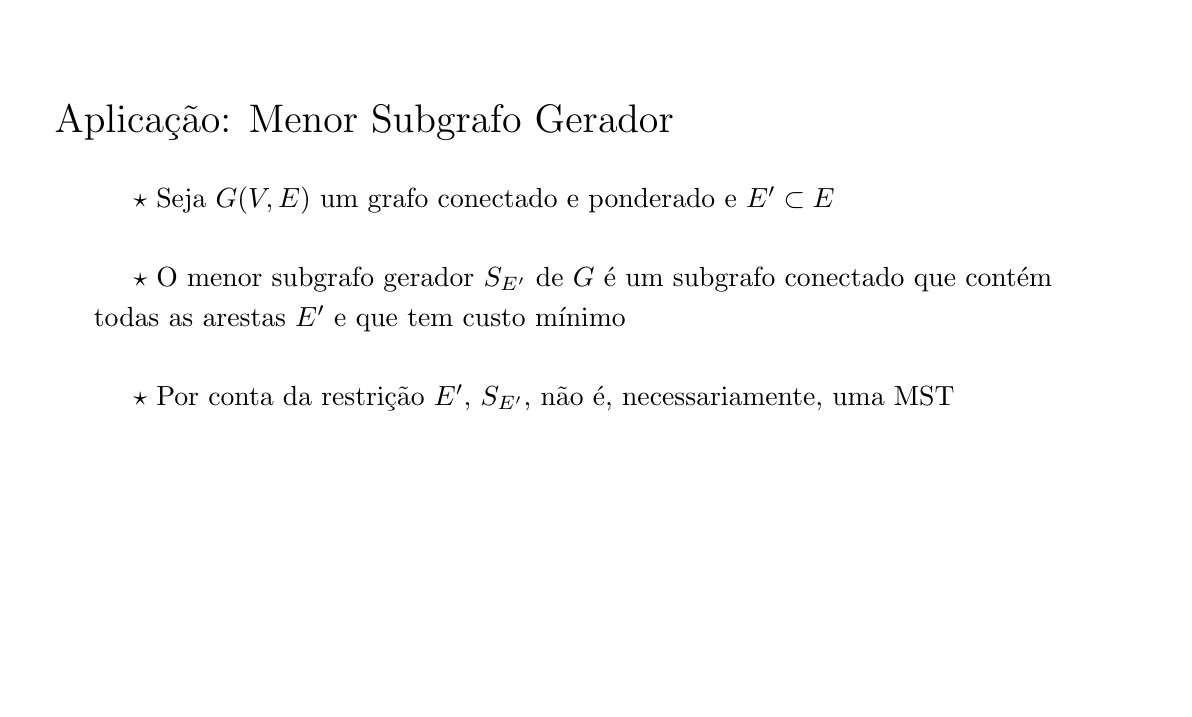
\begin{tikzpicture}
\node[draw,opacity=0] at (0, 0) {x};
\node[draw,opacity=0] at (14, 8) {x};

	\node[anchor=west] (title) at (0.0, 7.0) { \Large \bbbold{Aplicação: Menor Subgrafo Gerador} };


	\node[anchor=west] (a) at (1.0, 6.0) { $\star$ \bbtext{Seja $G(V, E)$ um grafo conectado e ponderado e $E'\subset E$} };


	\node[anchor=west] (b) at (1.0, 5.0) { $\star$ \bbtext{O menor subgrafo gerador $S_{E'}$ de $G$ é um subgrafo conectado que contém} };

	\node[anchor=west] (b1) at (0.5, 4.5) { \bbtext{todas as arestas $E'$ e que tem custo mínimo} };


	\node[anchor=west] (c) at (1.0, 3.5) { $\star$ \bbtext{Por conta da restrição $E'$, $S_{E'}$, não é, necessariamente, uma MST} };

\end{tikzpicture}
\end{frame}
\begin{frame}[plain,t]
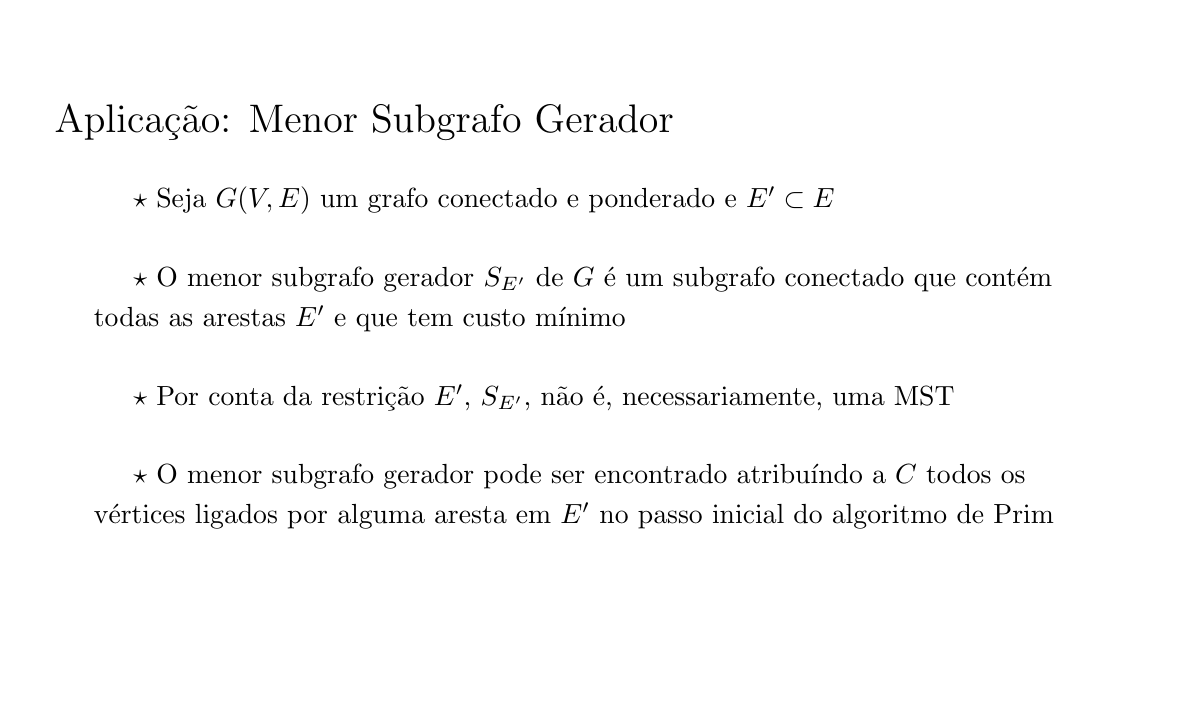
\begin{tikzpicture}
\node[draw,opacity=0] at (0, 0) {x};
\node[draw,opacity=0] at (14, 8) {x};

	\node[anchor=west] (title) at (0.0, 7.0) { \Large \bbbold{Aplicação: Menor Subgrafo Gerador} };


	\node[anchor=west] (a) at (1.0, 6.0) { $\star$ \bbtext{Seja $G(V, E)$ um grafo conectado e ponderado e $E'\subset E$} };


	\node[anchor=west] (b) at (1.0, 5.0) { $\star$ \bbtext{O menor subgrafo gerador $S_{E'}$ de $G$ é um subgrafo conectado que contém} };

	\node[anchor=west] (b1) at (0.5, 4.5) { \bbtext{todas as arestas $E'$ e que tem custo mínimo} };


	\node[anchor=west] (c) at (1.0, 3.5) { $\star$ \bbtext{Por conta da restrição $E'$, $S_{E'}$, não é, necessariamente, uma MST} };


	\node[anchor=west] (d) at (1.0, 2.5) { $\star$ \bbtext{O menor subgrafo gerador pode ser encontrado atribuíndo a $C$ todos os } };

	\node[anchor=west] (d1) at (0.5, 2.0) { \bbtext{vértices ligados por alguma aresta em $E'$ no passo inicial do algoritmo de Prim} };

\end{tikzpicture}
\end{frame}
\begin{frame}[plain,t]
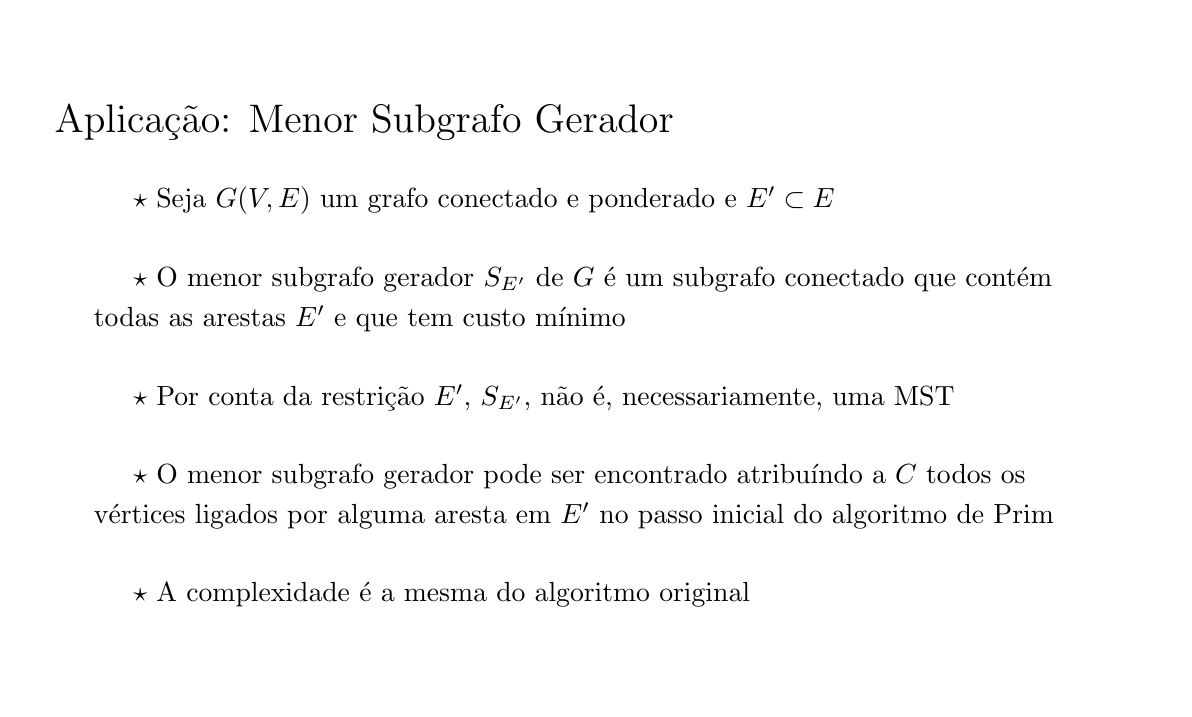
\begin{tikzpicture}
\node[draw,opacity=0] at (0, 0) {x};
\node[draw,opacity=0] at (14, 8) {x};

	\node[anchor=west] (title) at (0.0, 7.0) { \Large \bbbold{Aplicação: Menor Subgrafo Gerador} };


	\node[anchor=west] (a) at (1.0, 6.0) { $\star$ \bbtext{Seja $G(V, E)$ um grafo conectado e ponderado e $E'\subset E$} };


	\node[anchor=west] (b) at (1.0, 5.0) { $\star$ \bbtext{O menor subgrafo gerador $S_{E'}$ de $G$ é um subgrafo conectado que contém} };

	\node[anchor=west] (b1) at (0.5, 4.5) { \bbtext{todas as arestas $E'$ e que tem custo mínimo} };


	\node[anchor=west] (c) at (1.0, 3.5) { $\star$ \bbtext{Por conta da restrição $E'$, $S_{E'}$, não é, necessariamente, uma MST} };


	\node[anchor=west] (d) at (1.0, 2.5) { $\star$ \bbtext{O menor subgrafo gerador pode ser encontrado atribuíndo a $C$ todos os } };

	\node[anchor=west] (d1) at (0.5, 2.0) { \bbtext{vértices ligados por alguma aresta em $E'$ no passo inicial do algoritmo de Prim} };


	\node[anchor=west] (e) at (1.0, 1.0) { $\star$ \bbtext{A complexidade é a mesma do algoritmo original} };

\end{tikzpicture}
\end{frame}
\begin{frame}[plain,t]
\begin{tikzpicture}
\node[draw,opacity=0] at (0, 0) {x};
\node[draw,opacity=0] at (14, 8) {x};

	\node[draw,very thick,circle] (nodeA) at (4.0, 7.0) { \bbtext{A} };

	\node[draw,very thick,circle] (nodeB) at (10.0, 7.0) { \bbtext{B} };

	\node[draw,very thick,circle] (nodeC) at (13.0, 4.0) { \bbtext{C} };

	\node[draw,very thick,circle] (nodeD) at (7.0, 1.0) { \bbtext{D} };

	\node[draw,very thick,circle] (nodeE) at (1.0, 4.0) { \bbtext{E} };

	\draw[thick](nodeA) to node[above] { \footnotesize \bbinfo{1} } (nodeB);

	\draw[thick](nodeA) to node[above right] { \footnotesize \bbinfo{4} } (nodeC);

	\draw[thick,color=BBRed,dashed,very thick](nodeA) to node[below left,pos=0.2] { \footnotesize \bbinfo{4} } (nodeD);

	\draw[thick,color=BBRed,dashed,very thick](nodeA) to node[left] { \footnotesize \bbinfo{3} } (nodeE);

	\draw[thick](nodeB) to node[above right] { \footnotesize \bbinfo{5} } (nodeC);

	\draw[thick](nodeC) to node[below right] { \footnotesize \bbinfo{5} } (nodeD);

	\draw[thick](nodeC) to node[above, pos=0.3] { \footnotesize \bbinfo{2} } (nodeE);

	\draw[thick,color=BBRed,dashed,very thick](nodeD) to node[below left] { \footnotesize \bbinfo{3} } (nodeE);




\end{tikzpicture}
\end{frame}
\begin{frame}[plain,t]
\begin{tikzpicture}
\node[draw,opacity=0] at (0, 0) {x};
\node[draw,opacity=0] at (14, 8) {x};

	\node[draw,very thick,circle] (nodeA) at (4.0, 7.0) { \bbtext{A} };

	\node[draw,very thick,circle] (nodeB) at (10.0, 7.0) { \bbtext{B} };

	\node[draw,very thick,circle] (nodeC) at (13.0, 4.0) { \bbtext{C} };

	\node[draw,very thick,circle] (nodeD) at (7.0, 1.0) { \bbtext{D} };

	\node[draw,very thick,circle] (nodeE) at (1.0, 4.0) { \bbtext{E} };

	\draw[thick,color=BBCyan,dashed,very thick](nodeA) to node[above] { \footnotesize \bbinfo{1} } (nodeB);

	\draw[thick](nodeA) to node[above right] { \footnotesize \bbinfo{4} } (nodeC);

	\draw[thick,color=BBRed,dashed,very thick](nodeA) to node[below left,pos=0.2] { \footnotesize \bbinfo{4} } (nodeD);

	\draw[thick,color=BBRed,dashed,very thick](nodeA) to node[left] { \footnotesize \bbinfo{3} } (nodeE);

	\draw[thick](nodeB) to node[above right] { \footnotesize \bbinfo{5} } (nodeC);

	\draw[thick](nodeC) to node[below right] { \footnotesize \bbinfo{5} } (nodeD);

	\draw[thick](nodeC) to node[above, pos=0.3] { \footnotesize \bbinfo{2} } (nodeE);

	\draw[thick,color=BBRed,dashed,very thick](nodeD) to node[below left] { \footnotesize \bbinfo{3} } (nodeE);






\end{tikzpicture}
\end{frame}
\begin{frame}[plain,t]
\begin{tikzpicture}
\node[draw,opacity=0] at (0, 0) {x};
\node[draw,opacity=0] at (14, 8) {x};

	\node[draw,very thick,circle] (nodeA) at (4.0, 7.0) { \bbtext{A} };

	\node[draw,very thick,circle] (nodeB) at (10.0, 7.0) { \bbtext{B} };

	\node[draw,very thick,circle] (nodeC) at (13.0, 4.0) { \bbtext{C} };

	\node[draw,very thick,circle] (nodeD) at (7.0, 1.0) { \bbtext{D} };

	\node[draw,very thick,circle] (nodeE) at (1.0, 4.0) { \bbtext{E} };

	\draw[thick,color=BBCyan,dashed,very thick](nodeA) to node[above] { \footnotesize \bbinfo{1} } (nodeB);

	\draw[thick](nodeA) to node[above right] { \footnotesize \bbinfo{4} } (nodeC);

	\draw[thick,color=BBRed,dashed,very thick](nodeA) to node[below left,pos=0.2] { \footnotesize \bbinfo{4} } (nodeD);

	\draw[thick,color=BBRed,dashed,very thick](nodeA) to node[left] { \footnotesize \bbinfo{3} } (nodeE);

	\draw[thick](nodeB) to node[above right] { \footnotesize \bbinfo{5} } (nodeC);

	\draw[thick](nodeC) to node[below right] { \footnotesize \bbinfo{5} } (nodeD);

	\draw[thick,color=BBCyan,dashed,very thick](nodeC) to node[above, pos=0.3] { \footnotesize \bbinfo{2} } (nodeE);

	\draw[thick,color=BBRed,dashed,very thick](nodeD) to node[below left] { \footnotesize \bbinfo{3} } (nodeE);








\end{tikzpicture}
\end{frame}
\begin{frame}[plain,t]

\inputsnippet{cpp}{11}{30}{codes/msg.cpp}

\end{frame}
\begin{frame}[plain,t]

\inputsnippet{cpp}{31}{48}{codes/msg.cpp}

\end{frame}
\begin{frame}[plain,t]
\begin{tikzpicture}
\node[draw,opacity=0] at (0, 0) {x};
\node[draw,opacity=0] at (14, 8) {x};

	\node[anchor=west] (title) at (0.0, 6.0) { \Large \bbbold{Problemas sugeridos} };

	\node[anchor=west] (a) at (1.0, 5.0) { $1.$ \bbtext{CSES 1675 -- Road Reparation} };

	\node[anchor=west] (b) at (1.0, 4.0) { $2.$ \bbtext{OJ 10048 -- Audiophobia} };

	\node[anchor=west] (c) at (1.0, 3.0) { $3.$ \bbtext{OJ 10099 -- Tourist Guide} };

	\node[anchor=west] (d) at (1.0, 2.0) { $4.$ \bbtext{SPOJ IITKWPCG -- Help the old King} };

\end{tikzpicture}
\end{frame}
\begin{frame}[plain,t]
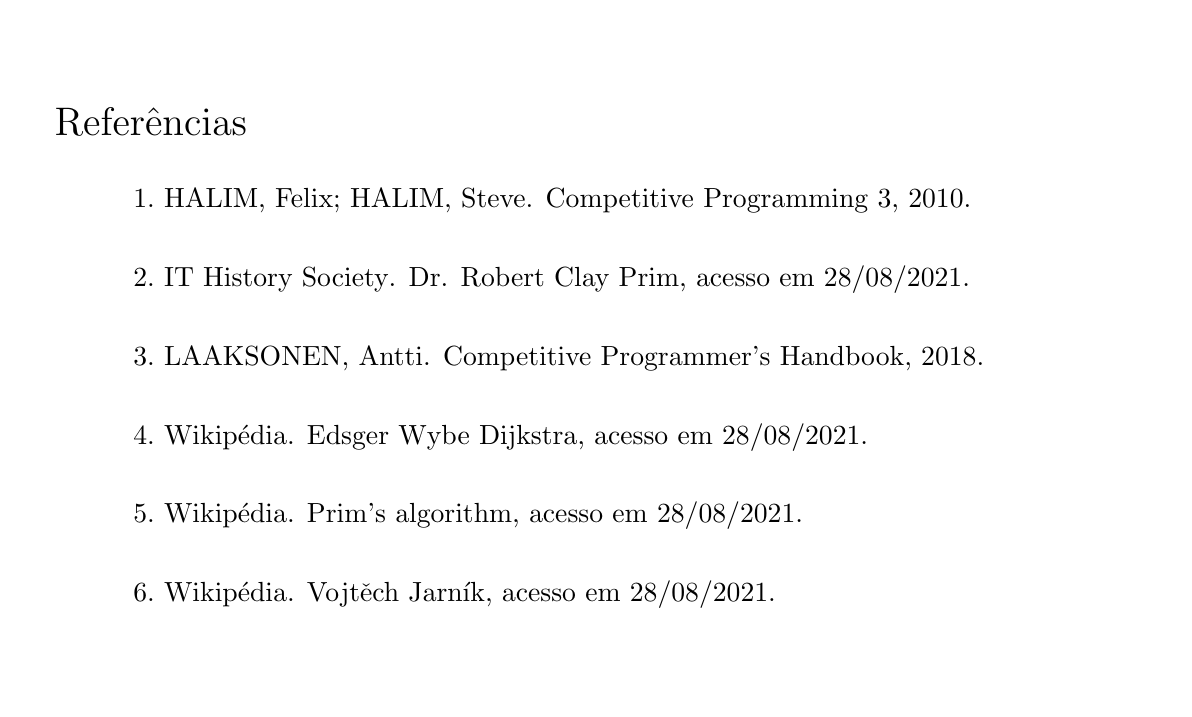
\begin{tikzpicture}
\node[draw,opacity=0] at (0, 0) {x};
\node[draw,opacity=0] at (14, 8) {x};

	\node[anchor=west] (title) at (0.0, 7.0) { \Large \bbbold{Referências} };

	\node[anchor=west] (a) at (1.0, 5.0) { $2.$ \bbtext{\bbbold{IT History Society}. \bbenglish{Dr. Robert Clay Prim}, acesso em 28/08/2021.} };

	\node[anchor=west] (b) at (1.0, 6.0) { $1.$ \bbbold{HALIM}, \bbtext{Felix}; \bbbold{HALIM}, \bbtext{Steve}. \bbenglish{Competitive Programming 3,} \bbtext{2010.} };

	\node[anchor=west] (c) at (1.0, 4.0) { $3.$ \bbbold{LAAKSONEN}, \bbtext{Antti}. \bbenglish{Competitive Programmer's Handbook,} \bbtext{2018.} };

	\node[anchor=west] (d) at (1.0, 3.0) { $4.$ \bbbold{Wikipédia}. \bbenglish{Edsger Wybe Dijkstra,} \bbtext{acesso em 28/08/2021.} };

	\node[anchor=west] (e) at (1.0, 2.0) { $5.$ \bbbold{Wikipédia}. \bbenglish{Prim's algorithm,} \bbtext{acesso em 28/08/2021.} };

	\node[anchor=west] (f) at (1.0, 1.0) { $6.$ \bbbold{Wikipédia}. \bbenglish{Vojtěch Jarník,} \bbtext{acesso em 28/08/2021.} };

\end{tikzpicture}
\end{frame}
\end{document}
